\chapter{A recurrent neural network for figure-ground organization of natural scenes}
\label{sec:natural_image}
\chaptermark{Figure-ground organization of natural scenes}

\section{Introduction}

Figure-ground organization is critical for visual understanding of the world around us. The process typically involves some form of segmentation, or dividing the input image into regions corresponding to objects and background. The border between any two regions is usually ``owned" by a single object, and the correct assignment of each border to its corresponding object is thought to be a precursor to scene understanding. However, this task is difficult due to the clutter, occlusion, and wide variety of features present in natural scenes. This problem has long fascinated researchers, including those from the fields of psychology~\citep{Wertheimer23,Koffka35}, neuroscience~\citep{Zhou_etal00,Craft_etal07}, and computer vision~\citep{Sajda_Finkel95,Ren_etal06,Teo_etal15,Wang_Yuille16}.
Despite this long line of research, our understanding of the neural basis of figure-ground organization remains surprisingly limited.

A key insight from neuroscience was the discovery of border-ownership
cells. Border-ownership selectivity is a property of a majority of the
neurons in V2, which encodes where an object is located relative to the
neuron's receptive field~\citep{Zhou_etal00}. When the edge of an object is presented in its receptive field (RF), a border-ownership cell will respond with different firing rates depending on where the object is located. For the example cell shown in Figure~\ref{Fig:experiments}A, objects placed to the upper right of the cell's RF (stimuli outlined in red) cause the cell to fire at a higher firing rate compared to objects placed to the lower left of the cell's RF (stimuli outlined in blue). Importantly, the local stimulus within the cell's RF is identical in both cases. Border-ownership coding has been studied using a wide variety of artificial stimuli, including those defined by luminance~\citep{Zhou_etal00}, motion~\citep{vonderHeydt_etal03a}, disparity~\citep{Qiu_vonderHeydt05}, and transparency~\citep{Qiu_vonderHeydt07}, and more recently, natural stimuli such as faces~\citep{Hesse_Tsao16,Ko_vonderHeydt17} and complex natural scenes~\citep{Williford_vonderHeydt16}.

\begin{figure}[t!]
\centering
\includegraphics[width=\textwidth]{NaturalImage/figs/exp_data.eps}
\makeatletter
\let\@currsize\normalsize
% simplify caption
\caption[Consistency of border-ownership coding across square and natural scene stimuli]{Consistency of border-ownership coding. (A) Border-ownership coding for an example cell. The cell has a preference for objects located to the upper right of its receptive field (RF) on both the square and natural scene stimuli, as indicated by higher firing rates. Red circles indicate the size and location of the cell's RF. Stimuli with objects to the upper right of the cell's RF (``preferred" side) are outlined in red, while stimuli with objects to the lower left of the cell's RF (``non-preferred" side) are outlined in blue. The cell's postimulus time histogram (PSTH) for the preferred side is shown by the red trace, while the PSTH for the non-preferred side is shown by the blue trace. Shading indicates 95\% confidence intervals. (B) Across the entire population of recorded cells, the mean border-ownership signal (difference in firing rate for the preferred and non-preferred sides) is similar for natural scenes and for squares, suggesting a common, robust cortical grouping mechanism. Panels A and B are modified from Figure 2 and Figure 6, respectively, of~\citet{Williford_vonderHeydt16}.}
\label{Fig:experiments}
\end{figure}

To explain this phenomenon, some computational models assume that
border-ownership coding is achieved purely by feedforward mechanisms, such as the asymmetric organization of surrounds \citep{Nishimura_Sakai04,Nishimura_Sakai05,Sakai_etal12} or global surround inhibition~\citep{Super_etal10}. Pure feedforward models predict similar latencies of the border-ownership signal regardless of the stimulus, but recent results show that border-ownership assignment of stimuli with illusory contours is delayed by $\sim30$ms compared to full stimuli~\citep{Hesse_Tsao16}. Other models propose  propagation of neural activity along horizontal connections within early visual
areas using a diffusion-like process \citep{Grossberg94,Sajda_Finkel95,
Baek_Sajda05, Kikuchi_Akashi01, Pao_etal99,Zhaoping05,Zucker12}. However, these models have difficulties explaining the fast establishment of border ownership which appears about 25ms after
the first stimulus response \citep{Zhou_etal00}.  Propagation along horizontal fibers over the distances used in the experiments would imply a delay of at least $\sim70$ms \citep[][based on the conduction velocity of horizontal fibers in primate V1 cortex; we are not aware of corresponding data for V2]{Girard_etal01}. Furthermore, such models are difficult to reconcile with the observation that the time course of border-ownership coding is largely independent of figure
size~\citep{Sugihara_etal11}.

An alternative computational model involves populations of grouping
($\mathcal{G}$) cells which explicitly represent (in their firing rates) the perceptual organization of the visual scene~\citep{Craft_etal07,Mihalas_etal11b}. These cells are reciprocally connected to border-ownership selective ($\mathcal{B}$) cells through feedforward and feedback connections. The combined activation of grouping cells and cells signaling local features represents the presence of a ``proto-object''~\citep[we borrow this term from the perception literature;][]{Rensink00a}. The use of proto-objects results in a structured perceptual organization of the scene. This proto-object based approach is consistent with psychophysical and neurophysiological studies
\citep[\eg][]{Duncan84,Egly_etal94,Scholl01,Kimchi_etal07,Qiu_etal07,Ho_Yeh09,Poort_etal12}. A feedforward version of this model has been applied to natural scenes, where it outperformed other models in predicting the locations of human eye fixations~\citep{Russell_etal14}.

A substantial fraction of neurons show consistent border-ownership coding across natural scenes that matches their preference on artificial stimuli, with the timing of border-ownership signals being similar for both types of stimuli (Figure~\ref{Fig:experiments}B). However, with the exception of a single computational model~\citep{Sakai_etal12}, we are not aware of any models that have quantitatively tested border-ownership selectivity on natural scenes. Here, we propose a model based on recurrent connections that is able to explain border-ownership coding in natural scenes. We compare our model results with experimental results, and find a good match both in the timing of the border-ownership signals as well as the consistency of border-ownership coding across scenes. In order to compare our model with other computer vision approaches, we also benchmarked our model on a standard contour detection and figure-ground assignment dataset~\citep{Martin_etal01} and achieve performance comparable to these other approaches.

\begin{figure}[t!]
\centering
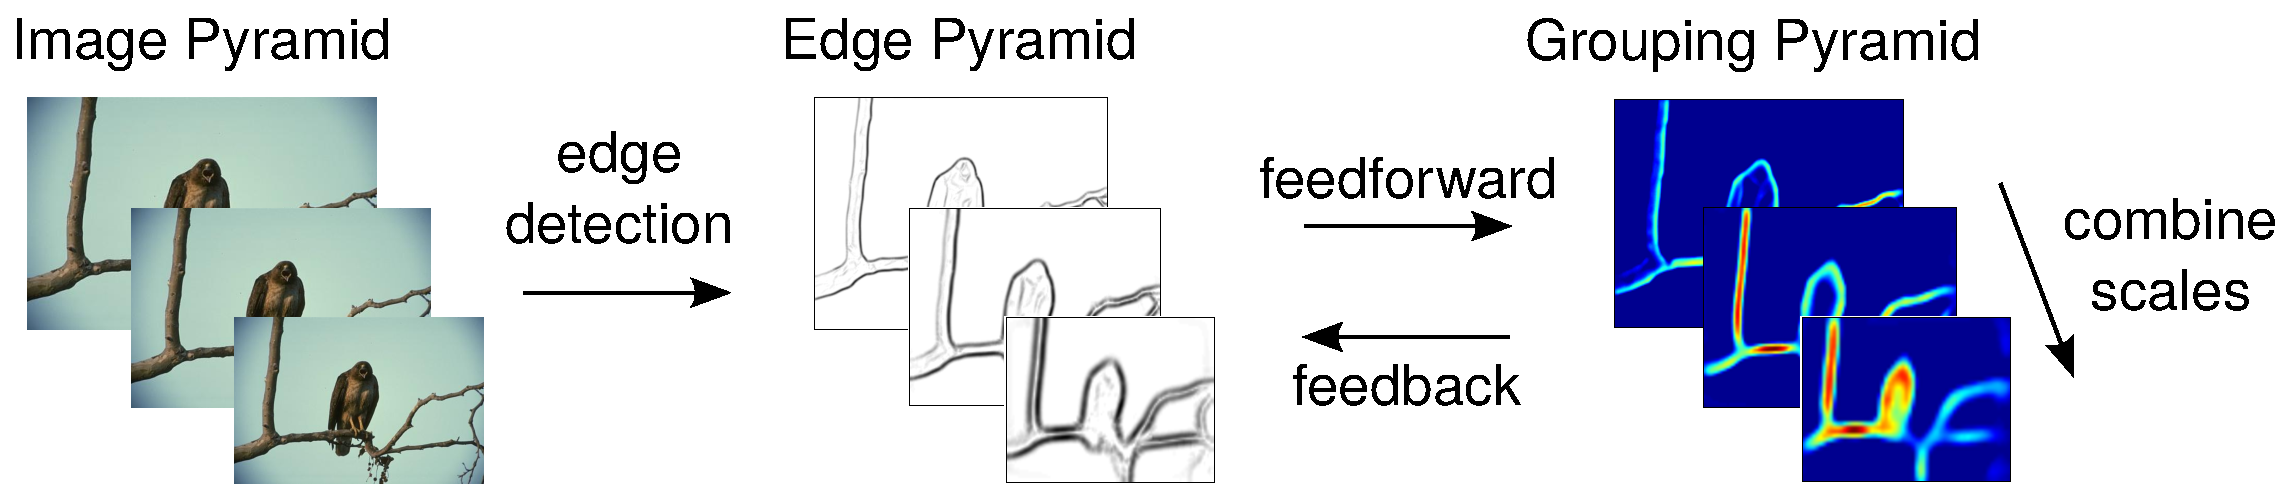
\includegraphics[width=\textwidth]{NaturalImage/figs/model_scheme_new.eps}
\makeatletter
\let\@currsize\normalsize
% simplify caption
\caption[Overview of the model for figure-ground organization of natural scenes]{Overview of the model. The image is first successively downsampled in half-octaves to create an image pyramid (only three scales are shown). The same set of feedforward and feedback grouping operations is then applied at each level of the pyramid to achieve scale invariance. Feedback from grouping cells is combined across scales so that global context information can influence figure-ground segmentation. The model is run for a total of 10 iterations (one iteration includes a feedforward and a feedback pass through the model), and our final results are based on neural activity from the highest resolution scale of the image pyramid.}
\label{Fig:model_overview}
\end{figure}

\section{Methods} 
\label{sec:model}
\subsection{Model Structure}

Our approach is an extension of the proto-object based model of saliency proposed by~\cite{Russell_etal14} and includes recurrent connections for figure-ground assignment. At the core of our model is a grouping mechanism which estimates figure-ground assignment within the input image using proto-objects of varying spatial scales and feature types. These proto-objects provide a coarse segmentation of the image through perceptual organization of the scene into regions corresponding to objects and background.
 
To achieve scale invariance, the algorithm successively downsamples the input image in steps of $\sqrt2$ to form an image pyramid spanning five octaves (Figure~\ref{Fig:model_overview}). The $k$th level of the pyramid is denoted using the superscript $k$. Unless explicitly stated, any operation applied to the pyramid is applied independently to each level and each feature type. Each layer of the network represents neural activity, which can either be propagated from one layer to another via feedforward or feedback connections since our model is recurrent. We use a filter-based approach, where the receptive fields of neurons are described by kernels and the correlation operation is used to calculate the neural response to an input. The model was implemented using MATLAB (Mathworks, Natick, MA,
USA).

The first stage of the model extracts edges from the input image based on either luminance or color information (Figure~\ref{Fig:model_overview}). We use the combination of receptive fields (CORF) operator, which is a model of V1 simple cells with push-pull inhibition~\citep{Azzopardi_etal14}. We chose the CORF operator due to its texture suppression properties, which can be beneficial when applied to natural images. Our model does not require a specific edge detection method and could be modified to use other front-end edge detectors (\eg Gabor filters). In the following, we only describe model computations on the luminance channel, but the exact same computations are also performed on the two color channels (\ie red-green and blue-yellow). As in~\citet{Russell_etal14}, the color channels were computed according to the methods outlined in the original~\citet{Itti_etal98a} visual saliency model.

For a given scale $k$, the output of the edge detection stage of the model are simple ($\mathcal{S}$) cells of eight different orientations $\theta$ and two contrast polarities, termed $\mathcal{S}^k_{\theta,L}(x,y)$ and $\mathcal{S}^k_{\theta,D}(x,y)$ (\ie for light-dark edges $L$ and dark-light edges $D$). For the two color channels, the edge polarities are determined by color-opponent responses (\eg red-green edges and green-red edges). Only the signal strength at the optimal orientation at each spatial location was used as input to the network. This simplification significantly reduces computation time by eliminating the calculation of responses for the non-optimum orientations.

In contrast to previous approaches which combine simple cell responses into a contrast-invariant complex cell response~\citep{Russell_etal14}, we keep the contrast-sensitive
$\mathcal{S}$ cell responses as they provide an informative cue for grouping along object edges. Objects tend to maintain similar contrast polarity along their boundaries, which may be useful for accurately determining figure-ground relationships. As a result, we have two sets of responses at each layer of our network corresponding to the two different types of contrast polarity.

Next, for a given angle~$\theta$, each $\mathcal{S}$ cell feeds into an opposing pair of border-ownership ($\mathcal{B}$) cells. As a result, $\mathcal{B}$ cells are also sensitive to contrast polarity, which is consistent with experimental findings~\citep{Zhou_etal00}.
For each contrast polarity, we used one-to-one connections between $\mathcal{S}$ cells of one orientation and the corresponding pair of
$\mathcal{B}$ cells with the same preferred orientation, but opposing side-of-figure preferences.
\begin{equation}
\begin{split}
\mathcal{B}^k_{\theta,L} = \mathcal{S}^k_{\theta,L}(x,y)\\
\mathcal{B}^k_{\theta+\pi,L} = \mathcal{S}^k_{\theta,L}(x,y)
\end{split}
\end{equation}
\begin{equation}
\begin{split}
\mathcal{B}^k_{\theta,D} = \mathcal{S}^k_{\theta,D}(x,y)\\
\mathcal{B}^k_{\theta+\pi,D} = \mathcal{S}^k_{\theta,D}(x,y)
\end{split}
\end{equation}

To infer whether the edges in $\mathcal{B}^k_{\theta,L}(x,y)$ and $\mathcal{B}^k_{\theta,D}(x,y)$ belong to figure or ground, knowledge of proto-objects in the scene is required. This context information is retrieved from a grouping mechanism (Figure~\ref{Fig:model_overview}). Grouping cells ($\mathcal{G}$) integrate information from $\mathcal{B}$
cells, and either respond to light objects on dark backgrounds, $\mathcal{G}^k_{L}(x,y)$, or dark objects on light backgrounds, $\mathcal{G}^k_{D}(x,y)$. This computation is similar to the use of center-surround cells in a feedforward version of the model~\citep{Russell_etal14}. In contrast to their approach, our model does not require an additional class of center-surround cells, but instead allows $\mathcal{G}$ cells to directly integrate local feature information from $\mathcal{B}$ cells and then bias the activity of these same cells using reciprocal feedback connections. Our model runs in an iterative manner, with one iteration corresponding to a feedforward and feedback pass through the model. $\mathcal{G}$ cell activity is combined across scales before each feedback pass, which allows the model to more accurately determine figure-ground assignment in a scale-invariant manner (Figure~\ref{Fig:model_overview}).

\begin{figure}[t!]
\centering

\includegraphics[width=\textwidth]{NaturalImage/figs/model_circuit.png}
\makeatletter
\let\@currsize\normalsize
% simplify caption
\caption[Structure of the recurrent neural network model for figure-ground organization of natural scenes]{Structure of the recurrent neural network. Each circle stands for a population of neurons with similar receptive fields and response properties. Red and blue lines represent excitatory and inhibitory projections, respectively. Solid and dashed lines represent purely feedforward and reciprocal feedforward/feedback connections, respectively. Edges and other local features of a figure (black square outline) activate simple cells ($\mathcal{S}$) whose receptive fields are shown by green ellipses. $\mathcal{S}$ cells project to border-ownership cells ($\mathcal{B}$) that have the same preferred orientation and retinotopic position as the $\mathcal{S}$ cells they receive input  from. However, for each location and preferred orientation there are  two $\mathcal{B}$ cell populations with opposite side-of-figure preferences, in the example shown $\mathcal{B}_{\pi}$ whose neurons respond preferentially when the foreground object is to the left of their receptive fields and $\mathcal{B}_{0}$ whose members prefer the foreground to the right side of their receptive fields. $\mathcal{B}$ cells have reciprocal, feedforward excitatory and feedback modulatory connections with grouping cells, $\mathcal{G}$, which integrate global context information about objects. The receptive field of a $\mathcal{G}$ cell is shown by the purple annulus. Opposing $\mathcal{B}$ cells compete indirectly {\em via} feedback inhibition  from $\mathcal{G}$ cells, which bias their activity and thus generate the border-ownership signal used to determine figure-ground assignment.}
\label{Fig:model}
\end{figure}

A more detailed view of the structure of our model is shown in Figure~\ref{Fig:model}. $\mathcal{G}$ cells integrate the $\mathcal{B}$ cell activity in an annular fashion. This allows $\mathcal{G}$ cells to show preference for objects whose borders exhibit the Gestalt principles of continuity and proximity. $\mathcal{G}$ cell activity is defined according to
\begin{equation}
\begin{split}
\mathcal{G}_{L}^k(x,y) = &\Bigg\lfloor\sum_\theta
                     [\mathcal{B}^k_{\theta,L}(x,y)-\mathcal{B}^k_{\theta+\pi,L}(x,y)]\ast v_\theta(x,y)\Bigg\rfloor
\end{split}
\label{eq:G_L}
\end{equation}
\begin{equation}
\begin{split}
\mathcal{G}_{D}^k(x,y) = &\Bigg\lfloor\sum_\theta
                     [\mathcal{B}^k_{\theta,D}(x,y)-\mathcal{B}^k_{\theta+\pi,D}(x,y)]\ast v_\theta(x,y)\Bigg\rfloor
\end{split}
\label{eq:G_D}
\end{equation}
where $\lfloor \cdot \rfloor$ is a half-wave rectification, and $\ast$ is the correlation operator defined as

\begin{equation}
f(x,y)\ast g(x,y) = \sum_{m=-\infty}^{\infty}\sum_{n=-\infty}^{\infty}f(m,n)g(x+m,y+n)
\end{equation}

$v_{\theta}$ is generated using the von Mises distribution as follows
\begin{equation}
v_\theta(x,y) = \frac{\exp\left[(\sqrt{x^2+y^2}-R_0)\cos(\tan^{-1}(\frac{y}{x})-\theta+\frac{\pi}{2})\right]}{2\pi I_0(\sqrt{x^2+y^2}-R_0)}
\label{eq:vonMises}
\end{equation}
where $R_0$ is the radius of the grouping cell receptive field, set to 2 pixels, and $\theta$ is the desired angle of the mask. The factor $\frac{\pi}{2}$ rotates the mask to ensure it is correctly aligned with the edge cells. $I_0$ is the modified Bessel function of the first kind. $v_\theta$ is then normalized according to
\begin{equation}
v_\theta(x,y) = \frac{v_\theta(x,y)}{\max(v_\theta(x,y))}
\end{equation}

On the first iteration, since there is no difference in activity between each pair of $\mathcal{B}$ cells as they receive the same initial bottom-up input, we omit the inhibition by the non-preferred
$\mathcal{B}$ cells and only use the activity of the preferred
$\mathcal{B}$ cells (eqs.~\ref{eq:G_L} and~\ref{eq:G_D}). On subsequent iterations, we include the inhibitory term. We also implement a simple form of local inhibition between the two grouping pyramids, $\mathcal{G}^k_{L}(x,y)$ and $\mathcal{G}^k_{D}(x,y)$. At each spatial location, only one type of $\mathcal{G}$ cell should be active, representing either a light or dark object at that location. For each level of the pyramid $k$, we perform a max operation as follows
\begin{equation}
	\mathcal{G}^k_{L}(x,y)=
	\begin{cases}
	\mathcal{G}^k_{L}(x,y) \:\;&if\;\mathcal{G}^k_{L}(x,y) > \mathcal{G}^k_{D}(x,y)\\
	0\;&otherwise
	\end{cases}\\
\end{equation}
\begin{equation}
	\mathcal{G}^k_{D}(x,y)=
	\begin{cases}
	\mathcal{G}^k_{D}(x,y) \:\;&if\;\mathcal{G}^k_{D}(x,y) > \mathcal{G}^k_{L}(x,y)\\
	0\;&otherwise
	\end{cases}\\
\end{equation}

Feedback from $\mathcal{G}$ cells to $\mathcal{B}$ cells is used to bias the responses of the $\mathcal{B}$ cells to correctly signal figure-ground assignment. The feedback depends on the contrast polarity of the $\mathcal{G}$ cell and the $\mathcal{B}$ cell. $\mathcal{B}^k_{\theta,L}$, the border-ownership activity for a light object on a dark background is given by
\begin{equation}
\begin{split}
\mathcal{B}^k_{\theta,L}(x,y) = &2\mathcal{S}^k_{\theta,L}(x,y)\\
            &\times\frac{1}{1+\exp\Big(-(\sum_{j\geq k}\frac{1}{2^{j-k}} v_{\theta+\pi}(x,y) \ast \mathcal{G}^j_{L}(x,y)-\sum_{j\geq k}\frac{1}{2^{j-k}} v_{\theta}(x,y) \ast \mathcal{G}^j_{D}(x,y))\Big)}
\end{split}
\label{eq:border-orientation1}
\end{equation}
and $\mathcal{B}^k_{\theta,D}$, the border-ownership activity for a dark object on a light background is given by
\begin{equation}
\begin{split}
\mathcal{B}^k_{\theta,D}(x,y) = &2\mathcal{S}^k_{\theta,D}(x,y)\\
            &\times\frac{1}{1+\exp\Big(-(\sum_{j\geq k}\frac{1}{2^{j-k}} v_{\theta+\pi}(x,y) \ast \mathcal{G}^j_{D}(x,y)-\sum_{j\geq k}\frac{1}{2^{j-k}} v_{\theta}(x,y) \ast \mathcal{G}^j_{L}(x,y))\Big)}
\end{split}
\label{eq:border-orientation2}
\end{equation}
where $v_{\theta}$ is the kernel responsible for mapping object activity in the grouping pyramids back to the objects edges, and the term $2^{-j}$ normalizes the $v_{\theta}$ operator across scales. The logistic function in the equations above enforces a form of competition between $\mathcal{B}$ cells such that their total activity is always conserved, and each $\mathcal{B}$ cell has activity between the range of zero and two times their initial bottom-up input activity, $\mathcal{S}^k_{\theta}(x,y)$.

In the equations above, feedback from $\mathcal{G}$ cells to $\mathcal{B}$ cells is contrast-sensitive. $\mathcal{B}$ cells receive excitatory feedback from $\mathcal{G}$ cells of the same contrast polarity on their preferred side and inhibitory feedback from $\mathcal{G}$ cells of the opposite contrast polarity on their non-preferred side. This is motivated by neurophysiological results which show that image fragments placed within the extra-classical receptive field of a border-ownership neuron can cause enhancement of the neuron's activity when placed on its preferred side, and suppression if placed on the non-preferred side \citep{Zhang_vonderHeydt10}. Furthermore, modulating the bottom-up $\mathcal{S}$ cell responses with $\mathcal{G}$ cell activity summed across spatial scales ensures that the $\mathcal{B}$ cell responses are scale-invariant. Neurophysiological results show border-ownership coding for stimuli of varying sizes, with the latency of the border-ownership signal being relatively independent of the size of the figure~\citep{Zhou_etal00,Sugihara_etal11}.

Figure-ground assignment should be robust for both light objects on dark backgrounds and dark objects on light backgrounds. In our model, this is achieved by computing $\mathcal{B}$ cell activity independently for each contrast polarity and then summing this activity to give a final border-ownership response independent of figure-ground contrast polarity. The $\mathcal{B}$ cell responses for light and dark objects are combined to give a contrast polarity invariant response
\begin{equation}
\mathcal{B}^k_{\theta}(x,y) =
\mathcal{B}^k_{\theta,L}(x,y)+\mathcal{B}^k_{\theta,D}(x,y)
\label{eq:BOS}
\end{equation}
The sign of the difference $\mathcal{B}^k_{\theta}(x,y)-\mathcal{B}^k_{\theta+\pi}(x,y)$ determines the direction of border ownership at pixel $(x,y)$ and orientation $\theta$. Its magnitude gives a confidence measure for the strength of border ownership.

Similarly, the $\mathcal{G}$ cell responses for light and dark objects are combined to give a contrast polarity invariant response
\begin{equation}
\mathcal{G}^k(x,y) =
\mathcal{G}^k_{L}(x,y)+\mathcal{G}^k_{D}(x,y)
\label{eq:G}
\end{equation}
The $\mathcal{G}$ pyramid from eq.~\ref{eq:G_L} and eq.~\ref{eq:G_D}, summed across both the light and dark channels, along with the figure-ground assignments in the $\mathcal{B}$ cells, is the output of the grouping algorithm and provides a perceptual organization of the visual scene.

As mentioned previously, we use both luminance and color information from the image in order to perform the grouping operation. The same exact operations that were performed on the luminance channel are also performed on the two color channels. We combine the final outputs of the $\mathcal{B}$ and $\mathcal{G}$ cells with an 80\% weighting for the luminance channel and a 10\% weighting for both the red-green and blue-yellow color channels. This choice of weighting does not qualitatively change our results.

\subsection{Model Implementation}
\label{sec:implementation}

All simulations were performed on a 300-core CPU cluster running Rocks 6.2 (Sidewinder), a Linux distribution intended for high-performance computing. This allowed us to independently run our model on different images, speeding up our testing time. We ran the model for a total of 10 iterations, with each iteration being one feedforward pass of $\mathcal{B}$ cell to $\mathcal{G}$ cell activity, followed by one feedback pass of $\mathcal{G}$ cell to $\mathcal{B}$ cell activity (Figure~\ref{Fig:model_overview}). We generally found that the model converged after only a few iterations. The final $\mathcal{G}$ cell activity was summed across scales. Contour detection and figure-ground assignment results are computed from the population of $\mathcal{B}$ cells at the highest resolution level of the image pyramid, which had the same resolution as the input image. $\mathcal{B}$ cell activity is converted into a population vector code by summing the final activity across orientations, where the magnitude of the resulting vector represents the border-ownership signal (or edge strength), and the direction of the vector provides a continuous figure-ground orientation label. For a given image, we normalize the border ownership signal at each pixel $(x,y)$ by the maximum border ownership signal across the entire image, such that the border ownership signal is bounded between -1 and 1.

We benchmarked our model on the publicly available Berkeley Segementation Dataset \citep{Martin_etal01}. We did this in the context of two tasks: contour detection and figure-ground assignment. Each dataset includes 100 to 200 test images, and we report F-scores (harmonic mean of precision and recall) for the contour detection task and mean accuracy (percent of correctly labeled figure-ground edges) for figure-ground assignment task averaged over all test images. We used publicly available benchmarking code to do our analysis and comparisons with other approaches.

\subsection{Model to Cell Comparison}
\label{sec:cell_model}
% Edit this section based on our final choice of analysis
To compare our model results with experimental results, we used a publicly available dataset of border-ownership cell responses recorded during viewing of natural scenes~\citep{Jonathan_data}. More details about the stimuli, experimental design, and data analysis can be found in the corresponding paper~\citep{Williford_vonderHeydt16}.
% Edit this accordingly...
The dataset includes border-ownership signals (BOS) for each scene that was viewed by each recorded cell. To perform our analyses, we calculated the model's border ownership signal for the same set of scenes shown to the cells. We quantified model performance by using a combination of the cosine similarity metric, statistical testing, and regression goodness of fit, which are explained in more detail below.
%
%We examined two aspects of the dataset. First, we looked at the model responses over a large numver of scenes as a means to estimate the model's consistency. Our results show the model's border ownership responses sorted across scenes.

\subsubsection{Cosine Similarity}
\label{sec:cos-sim-methods}
For our analyses, we first chose a subset of cells ($N=13$) from the population of recorded cells which had highly consistent border-ownership responses (defined as having the same sign of border ownership on $>$80\% of their tested scenes). To compare the BOS responses of a cell to another cell or a cell to the model on the set of common scenes viewed by both, we used the cosine similarity metric, which is defined as

\begin{equation}
\cos(\theta) = \frac{A \cdot B}{||A||_{2}||B||_{2}} = \frac{\sum\limits_{i=1}^{n}A_{i}B_{i}}{\sqrt{\sum\limits_{i=1}^{n}A_{i}^2}\sqrt{\sum\limits_{i=1}^{n}B_{i}^2}}
\label{eq:cos_sim}
\end{equation}
where $A_i$ and $B_i$ are components of the vectors $A$ and $B$ respectively.

In our case, we can treat the BOS responses of each cell and the model on a set of scenes as a vector in a high-dimensional space (with each axis being the BOS for one scene). We can then compute the cosine similarity between any two given vectors (\eg between one cell and another cell or between a cell and the model). The cosine similarity is bounded between -1 and 1, with the geometric interpretation that the metric measures the cosine of the angle between two vectors in a high-dimensional space. Two vectors which are exactly the same will have a cosine similarity of 1, two vectors that are exactly opposite will have a cosine similarity of -1, and a cosine similarity of 0 indicates two vectors that are orthogonal or decorrelated. We also explored using the Pearson correlation coefficient ($r$), but found that this metric often underestimated similarity due to the requirement of first mean centering the BOS responses.

\subsubsection{Bootstrap and Equivalence Testing}
\label{sec:equivalence_test}
To test the hypothesis that the model performs similarly to the most consistent cells from the experiment, we used a combination of bootstrap testing and equivalence testing on the cell-cell and cell-model cosine similarities computed above. To perform the bootstrap test, means of the cell-cell and cell-model cosine similarities were calculated using resampling with replacement under the null hypothesis that the cell-cell and cell-model cosine similarities come from the same distribution. We calculated the bootstrap estimate of the difference in the means using a total of $N = 10,000$ trials.

Equivalence testing is not as well known, but has traditionally been used in the bioequivalence setting, for example, to compare whether the efficacy of a new drug is similar to that of an existing drug on the market. In standard hypothesis testing, a possible null hypothesis is that the means of two distributions are not different in a statistically significant manner. However, failure to reject the null hypothesis is not sufficient proof to conclude that the two distributions are actually similar, as the test may also fail due to not having enough statistical power. In equivalence testing, the null hypothesis is instead that the means of the two distributions differ by a pre-determined ``zone of scientific indifference." The alternative hypothesis (where the burden of proof lies) is that the means of the two distributions fall within this zone and can thus be considered similar. In our case, the equivalence test is performed by either using two one-sided $t$-tests or computing confidence intervals on the difference in the means of the two distributions, and determining whether this confidence interval lies within the pre-determined zone of scientific indifference. We chose a zone between -0.2 and 0.2, which represents $\pm$10\% of the full range of possible cosine similarity values.

\subsubsection{Goodness of Fit}
In order to quantify model performance on a per-cell basis, we also performed linear regression on the cell's border-ownership responses across scenes (ordinate) against the model's border-ownership responses across the same set of scenes (abscissa). For each regression, we forced the least-squares line through the origin because the sign of the border-ownership signal for a given neuron is arbitrary. Two border-ownership selective neurons responding to the same edge can have opposite side-of-figure preferences, and which direction we assign a positive value to is arbitrary. As a result, the line of best fit must be invariant against reflecting any data points about the origin, which is why it must pass through the origin.

The linear regression provides a measure of the percentage of variance that can be explained by our model. However, each cell's response contains a repeatable component (in response to the same stimulus, which we attempt to capture with our model) and a noise component (which is completely random). Because our model is deterministic, it is unable to capture the noise component present in the cell responses.  We only care about the explainable variance, which is the total response variance minus the noise variance, where the noise variance can be estimated from a small number of stimulus presentations from the experiments. As a result, we defined our goodness of fit measure for the regression by computing the fraction of explainable variance that can actually be explained by the model

\begin{equation}
\text{goodness of fit} = \frac{\sigma^2_{explained}}{\sigma^2_{explainable}} = \frac{[\sigma^2_{predicted}-(1/N_{scenes})\sigma^2_{noise}]}{[\sigma^2_{response}-\sigma^2_{noise}]}
\label{eq:gof}
\end{equation}
where we apply a correction term in the numerator for the fraction of the noise variance captured by the regression. This is determined by the ratio of the degrees of freedom in the regression (1 for the slope of the line) to the degrees of freedom in the data (the number
of scenes, $N_{scenes}$). We follow the general methods put forth in~\citet{DiCarlo_etal98} for calculating this goodness of fit measure.

\section{Results}
\label{sec:results}

\subsection{Evaluation of the model on standard benchmarks}
% List which algorithms we compared against here
We benchmarked our model on the Berkeley Segmentation Dataset~\citep{Martin_etal01}. We did this for two separate tasks: 1) a contour detection task and 2) a figure-ground assignment task. Importantly, our model uses the same set of parameters for both tasks, and parameters were not tuned separately for each task. Examples of our model output are shown in Figure~\ref{Fig:results_summary}. We show the original input image, the edge maps, the border-ownership signals, and the final grouping maps. Although we did not specifically design our model to achieve good performance on the contour detection task, we hypothesized that the border-ownership signal is a good correlate of the perceptual saliency of object contours. As such, we use the border-ownership signal (independent of figure-ground orientation) as the model output for the contour detection task.

\begin{figure}[t!]
\centering
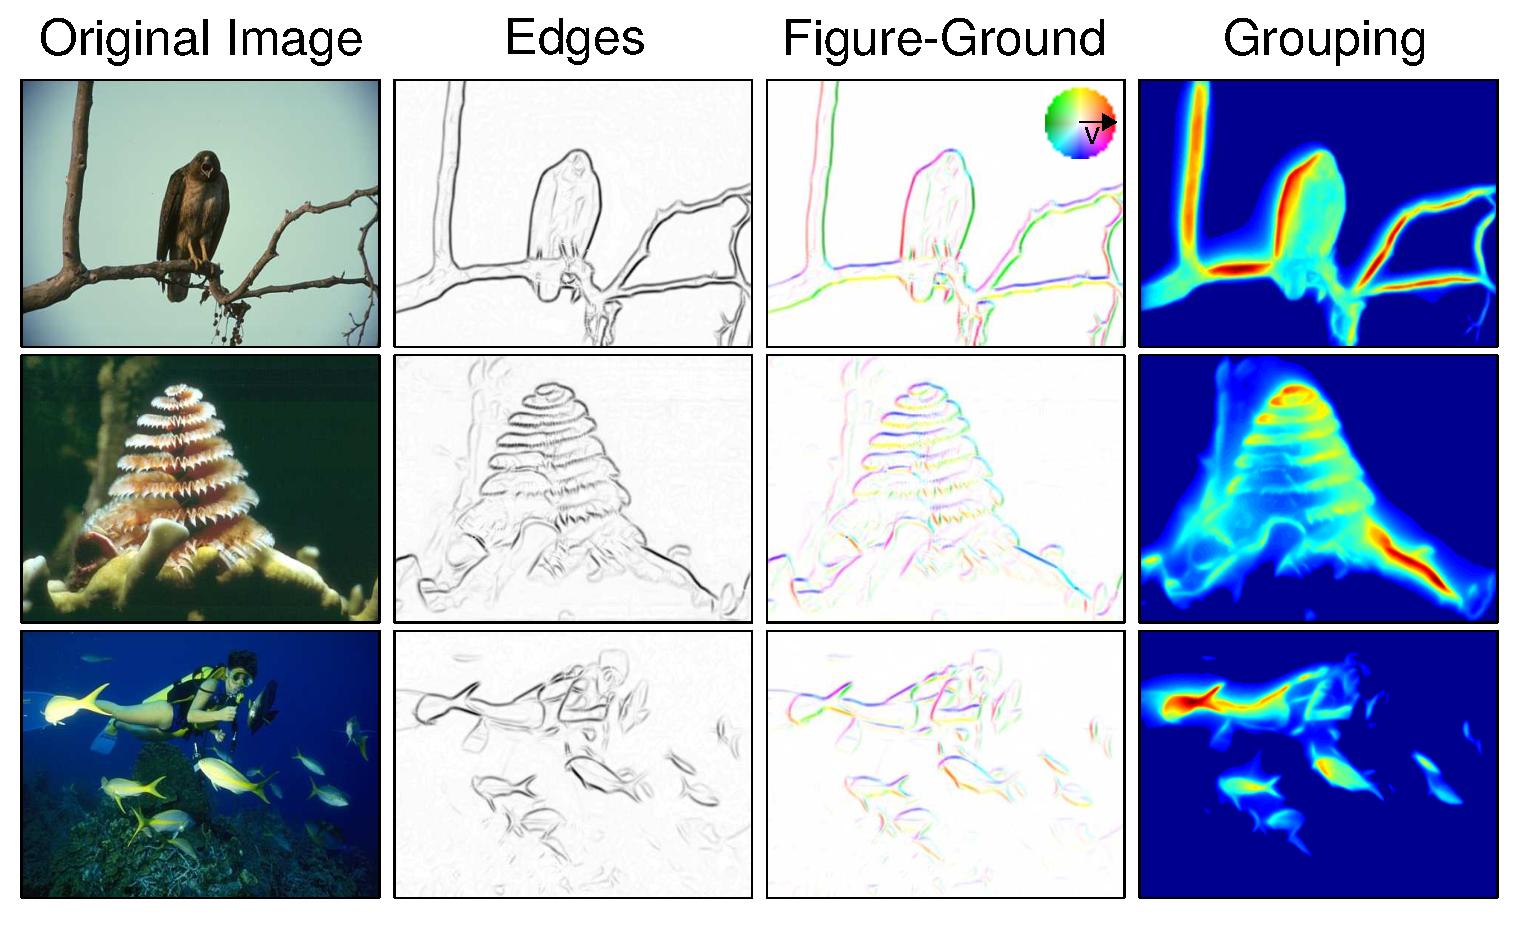
\includegraphics[width=\textwidth]{NaturalImage/figs/results_new}
\makeatletter
\let\@currsize\normalsize
% simplify caption
\caption[Model results on images from the BSDS dataset]{Results of our model on example images from the Berkeley Segmentation Dataset. Columns from left to right are the original images, the edge maps, the border-ownership cell activity (representing figure-ground assignment), and also grouping cell activity. For the figure-ground assignment, the color of each edge is represented by a hue and a saturation value (see color wheel insert). The hue of the edge represents the figure-ground orientation label with the arrow convention shown in the color wheel (\eg red represents an object pointing to the right) and the saturation of the edge represents the strength of the border-ownership signal.}
\label{Fig:results_summary}
\end{figure}

We quantify our results on the contour detection task using the F-score, which is the harmonic mean of the accuracy and precision of contour detection. For the contour detection task, we compare our model to three different approaches: ultrametric contour maps~\citep[][gPb-owt-ucm]{Arbeleaz_etal11}, structured edges~\citep[][SE]{Dollar_Zitnick15}, and structured random forests~\citep[][SRF]{Teo_etal15}. Overall, we achieved an F-score of 0.64 on the contour-detection task. State-of-the-art computer vision models achieve F-scores on the order of 0.73 (all three approaches gave similar results). Our model does not perform as well as these other approaches, which may be the result of limitations in the initial edge detection method we used in our model. Again, we did not design our model for the contour detection task, but we were able to use computed border-ownership signals from the model as a measure of contour detection strength.

%% Insert table of results here for contour detection and figure-ground
\begin{table}[h!]
\centering
\begin{tabular}{|c|c|c|c| } 
 \cline{2-4}
 \multicolumn{1}{c}{} & \multicolumn{3}{|c|}{\textbf{BSDS500}} \\
 \cline{2-4}
 \multicolumn{1}{c|}{} & ODS & OIS & AP\\ 
 \hline
 Human & 0.80 & 0.80 & -\\ 
 \hline
  Our approach & 0.64 & 0.65 & 0.51 \\
 gPb-owt-ucm & 0.73 & \textbf{0.76} & 0.73 \\
 SE & 0.73 & 0.75 & \textbf{0.77} \\
 SRF & 0.73 & 0.74 & 0.76 \\
 \hline
\end{tabular}
\makeatletter
\let\@currsize\normalsize
\caption[Contour detection results]{Contour-detection results. Numbers shown are the F-measures when choosing the optimal scale for the entire dataset (ODS) or per image (OIS), as well as the average precision (AP).}
\label{tbl:Table1}
\end{table}

\begin{table}[h!]
\centering
\begin{tabular}{|c|c|} 
 \cline{2-2}
 \multicolumn{1}{c}{} & \multicolumn{1}{|c|}{\textbf{BSDS}} \\
\cline{2-2}
 \multicolumn{1}{c|}{} & Mean Accuracy \\ 
 \hline
  Our approach & 71.5\% \\
 SRF & \textbf{74.7\%} \\
 Global-CRF & 68.9\% \\
 2.1D-CRF & 69.1\% \\
 \hline
\end{tabular}
\makeatletter
\let\@currsize\normalsize
\caption[Figure-ground assignment results]{Figure-ground assignment results. Numbers shown are the mean accuracy across all matched scene points.}
\label{tbl:Table2}
\end{table}

For the figure-ground assignment task, we quantify our results using the mean accuracy of figure-ground assignment across all labeled contours in the test images. The model's figure-ground label for a given scene point in the image is considered correct if it falls within $90^{\circ}$ of the true figure-ground label. We compared our model to structured random forests~\citep[][SRF]{Teo_etal15} and two conditional random field approaches, Global-CRF~\citep{Ren_etal06} and 2.1D-CRF~\citep{Leichter_Lindenbaum09}. Overall, we achieved a mean accuracy of 71.5\% on the figure-ground assignment task. Structured random forests achieve a higher mean accuracy of 74.7\%. Surprisingly, our model outperforms the two other approaches based on conditional random fields~\citep{Ren_etal06,Leichter_Lindenbaum09}, which achieved mean accuracies below 70\%. There is also a recent deep learning approach to the same problem~\citep{Wang_Yuille16}, but since the results of this method were not benchmarked using the above standard tests, we do not include it in our comparison.

Computer vision approaches are able to achieve better performance than our model based on the evaluation metrics described above, but require extensive training and parameter tuning, often on a held-out set of training images. In contrast, our model is built based on first principles and does not require any specific form of training. Although our model does not outperform the state-of-the-art, it does represent an alternative approach based on biologically plausible neural computations that require very little training or tuning of parameters.

We report our results on the contour detection and figure-ground assignment tasks in Tables~\ref{tbl:Table1} and \ref{tbl:Table2} above, respectively. All benchmarks were performed using public code made available by the authors of the original papers.

\begin{figure}[t!]
\centering
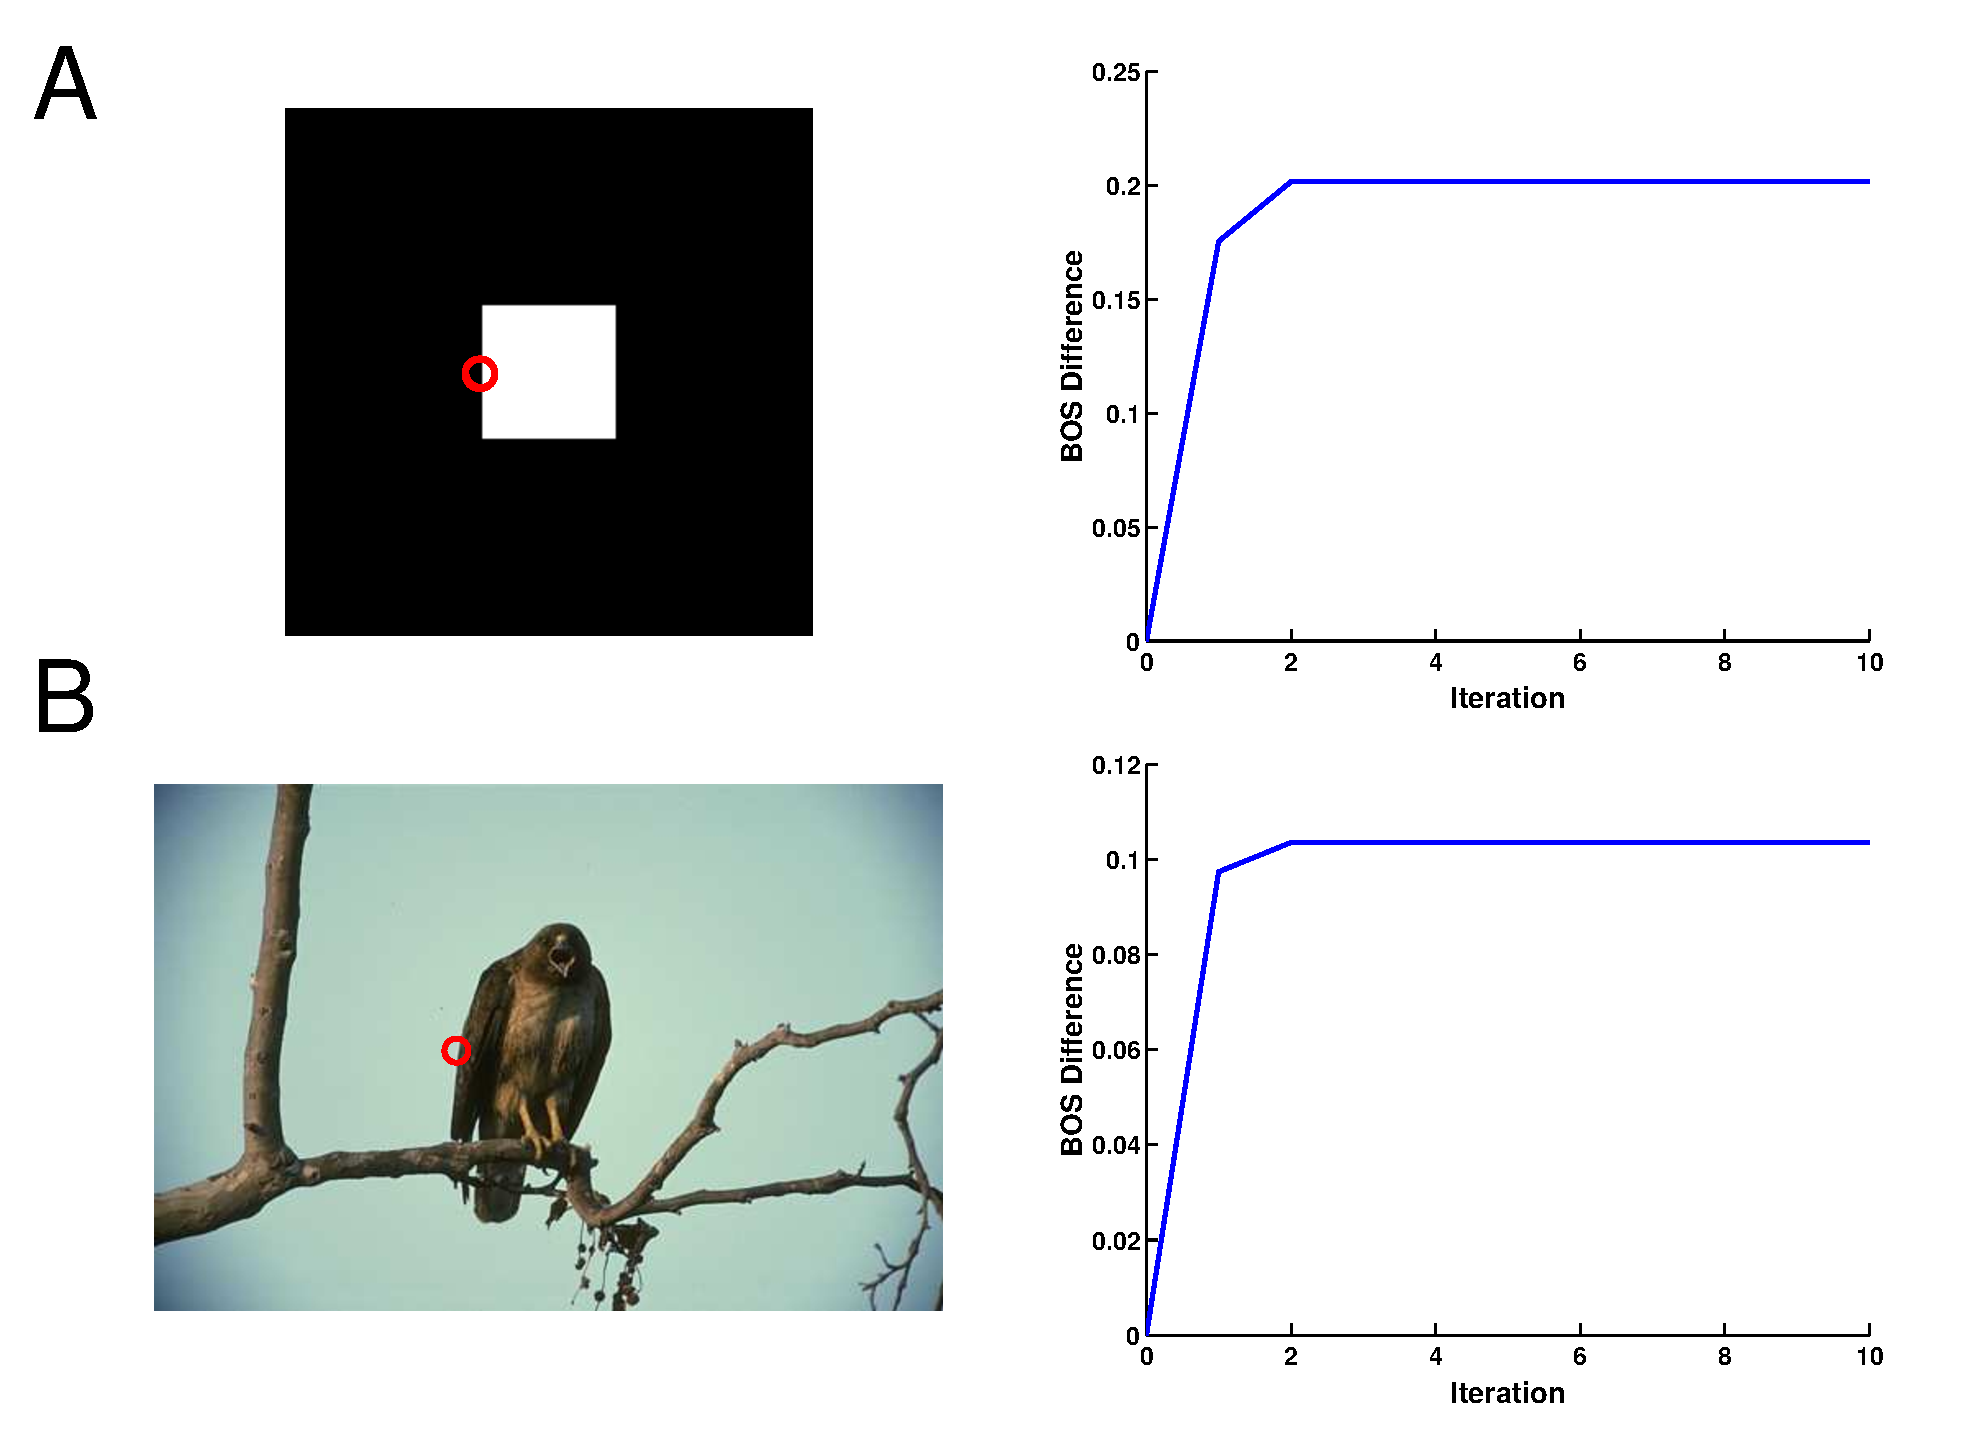
\includegraphics[width=\textwidth]{NaturalImage/figs/BOS_timecourse.eps}
\makeatletter
\let\@currsize\normalsize
% simplify caption
\caption[Time course of border-ownership coding]{Time course of border-ownership coding. The model converges to the correct border-ownership assignment within two-three iterations (one iteration corresponds to a feedforward and feedback pass through the model). The receptive field of the model's border ownership cell is shown by the red circle. The input image and time course of the border-ownership signal are shown for both the standard square commonly used in experiments (A) and an example natural scene from the Berkeley Segmentation Dataset (B). The border-ownership signal is computed as the difference in activity between the preferred and non-preferred border-ownership cells in the model.}
\label{Fig:results_time}
\end{figure}

\subsection{Timing of the border-ownership signal}
% What other results would be nice to show?
We tested our model on the standard square stimuli used to determine border-ownership preference in experiments~\citep{Zhou_etal00}, as well as a wide array of natural scenes from the Berkeley Segmentation Dataset. We found that our model converges within a few iterations, demonstrating that only a few feedforward and feedback passes are needed to determine figure-ground assignment for a given image (Figure~\ref{Fig:results_time}).
% more speculative here...
Given that white-matter projections in the brain are quite fast, we assume that a single feedforward and feedback pass in our model takes about 10 ms. As the model converges within 2-3 iterations, the border-ownership signal will reach its peak within 20-30 ms of the initial visual response. A similar time course has also been observed in the experimental data, with the border-ownership signal appearing approximately 30 ms after visual response onset~\citep{Williford_vonderHeydt16}.
%
The similar time course of BOS tuning on both artificial and natural stimuli suggests a common cortical mechanism for grouping, which is also supported by previous experimental results demonstrating consistent border-ownership coding across these different types of stimuli. Our model is able to reproduce this result, showing a similar time course for border-ownership coding on both the square and natural scene stimuli.
% Can we comment more on the timing similarity with Jonathan's data?

\begin{figure}[t!]
\centering
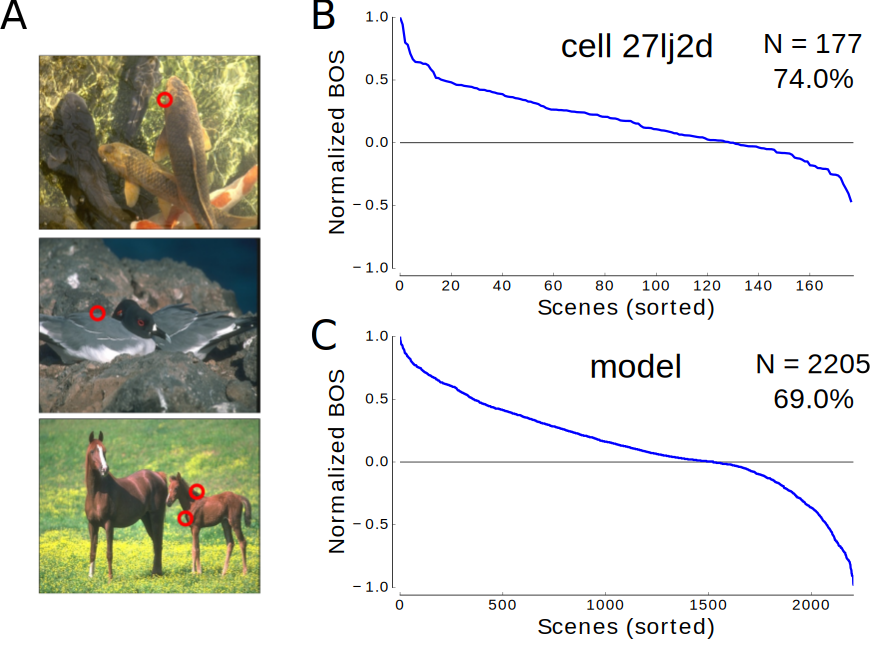
\includegraphics[width=\textwidth]{NaturalImage/figs/cell_model_consistency}
\makeatletter
\let\@currsize\normalsize
% simplify caption
\caption[Cell and model consistency across scenes]{Cell and model consistency across scenes. (A) Examples of scenes that were used to test border-ownership selectivity during the experiments. Red circles represent scene points within the images, which were centered on the receptive fields of border-ownership selective neurons during the experiments and during our testing of the model. A single image could contain multiple scene points, as shown by the example in the last row. (B) The normalized border-ownership signal (BOS) for example cell $27lj2d$ is shown according to each scene, with scenes sorted in decreasing order by strength of BOS. The cell achieved a consistency of 74.0\% across all tested scene points ($N = 177$). Consistency is defined as the number of scenes with positive border-ownership signal divided by the total number of scenes. (C) The normalized BOS signal for the model is shown with the same convention as in (B). The model achieved an overall consistency of 69.0\% across all tested scene points ($N = 2205$), consistent with our finding that the overall accuracy of the model is around 70\% on the figure-ground assignment benchmark.}
\label{Fig:cell_model_consistency}
\end{figure}

\subsection{Comparison of model results to experimental results}
% Display figure here related to these results
The model exhibits consistent border-ownership coding across a large number of natural scenes, similar to the most consistent cells from the experiment. Figure~\ref{Fig:cell_model_consistency} compares the border-ownership signals sorted in descending order by scene for an example cell and for the model. The example cell shows a consistency of 74.0\% across 177 scenes, which was the largest number of scenes that was tested for any single cell in the dataset. A large number of cells in the dataset were highly consistent, including the 13 cells we chose with $>$80\% consistency, and within this subset of cells, three cells with $>$90\% consistency. In comparison, the model shows a lower overall consistency of 69.0\% across 2205 tested scenes (the full set of scenes viewed by all the highly consistent cells). Although the model was tested with more than an order of magnitude more scenes than the example cell, it still remained highly consistent. This level of consistency is similar to the 70\% accuracy the model achieved on the figure-ground assignment benchmark, demonstrating the validity of the model.

We also used the cosine similarity metric (see Section~\ref{sec:cos-sim-methods}) to quantify similarity in BOS responses between cells and similarity between cells and the model on a shared set of scenes. Despite the large diversity in cells and their responses, we found that our model was able to largely explain the border-ownership coding of highly consistent cells on natural scenes.
% First show comparison of cell-cell and cell-model, then the full cell-model results?
%
Figure~\ref{Fig:cell_model_cos} shows the cell-model cosine similarities on a per-cell basis for the subset of highly consistent cells. The model-cell cosine similarities were all positive, ranging from 0.21 - 0.69, with a mean similarity of 0.44.

Given biological noise and inter-cell differences, we did not expect that the model-cell cosine similarities would reach unity. In order to characterize an upper bound on the cosine similarity values, we also calculated the cosine similarities between all pairs of highly consistent cells ($N = 58$ pairs). For the cell-cell comparisons, the cosine similarities ranged from 0.14-0.91, with a mean similarity of 0.54. 
% Add sentence on bootstrap
Bootstrap testing revealed no significant statistical difference between the means of the cell-cell and cell-model cosine similarities ($p = 0.15$).
%
As an additional statistical test, we also used equivalence testing (see Section~\ref{sec:equivalence_test}). Equivalence testing on the means of the cell-cell cosine similarities and model-cell cosine similarities revealed no difference in the mean values based on a zone of scientific significance between -0.2 and 0.2 ($p$ = 0.02). As a result, we conclude that our model performs similarly compared to the highly consistent cells in the dataset.

\begin{figure}[t!]
\centering
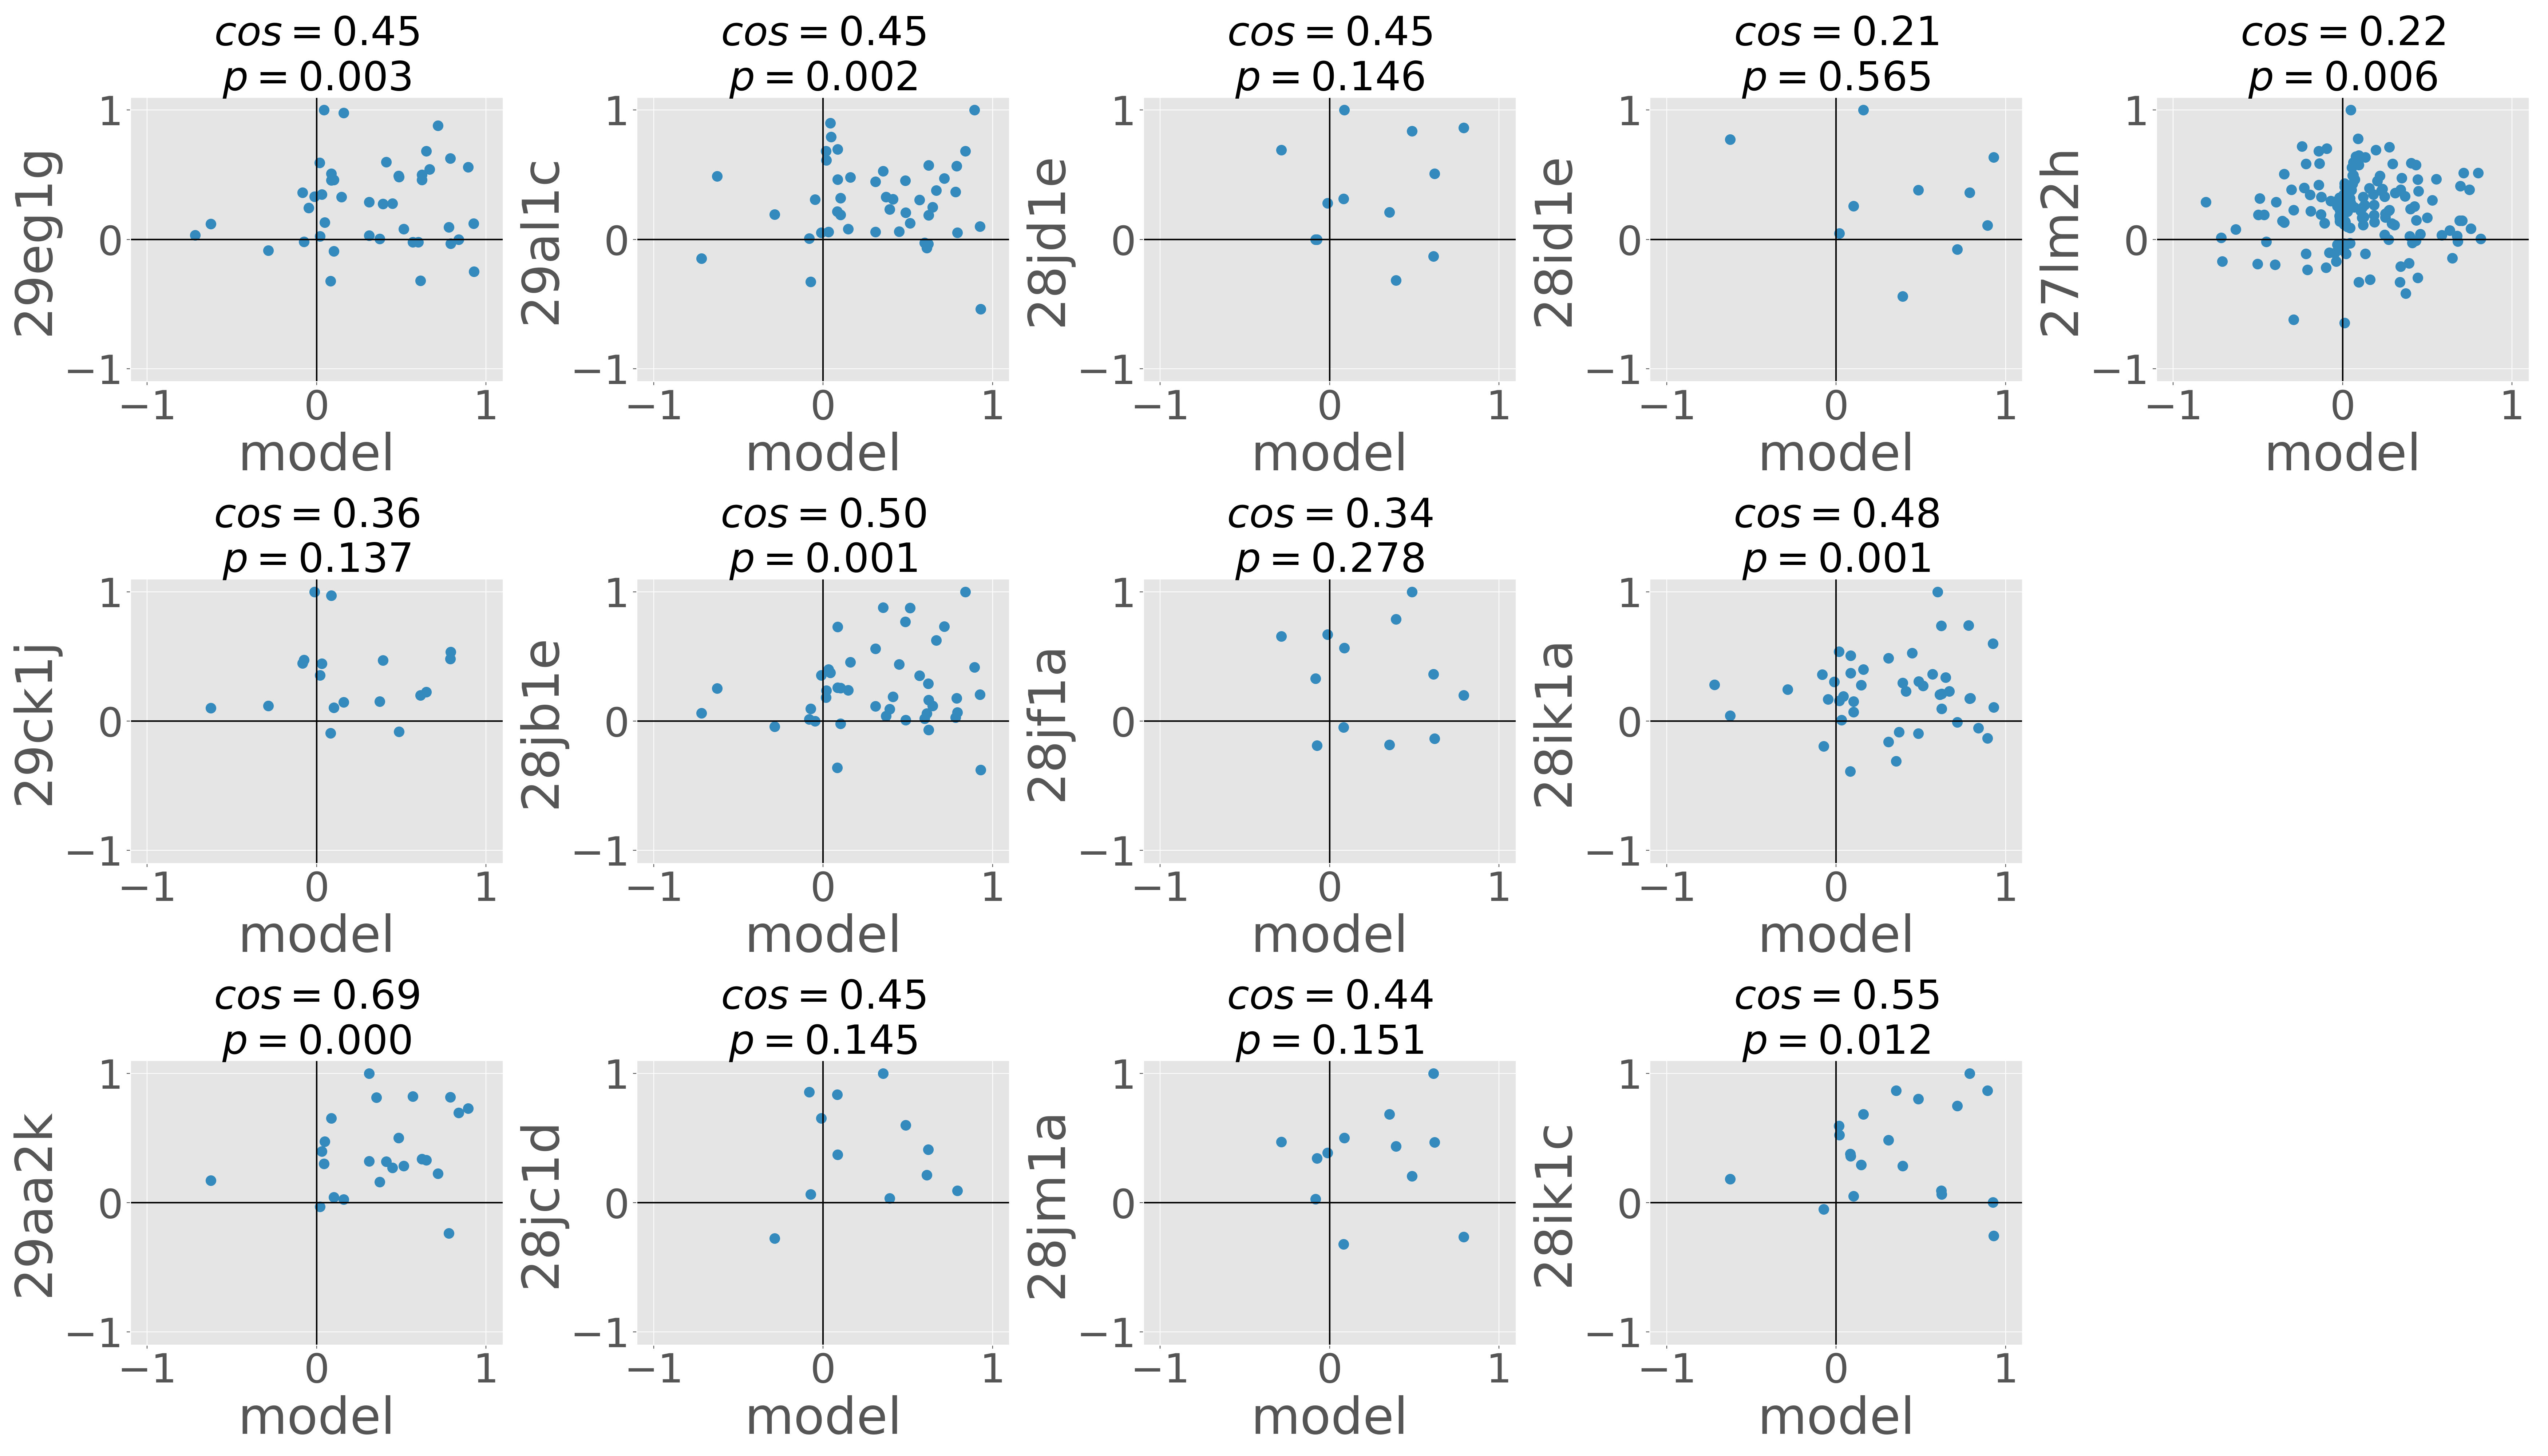
\includegraphics[width=\textwidth]{NaturalImage/figs/cell_model_cos_p}
\makeatletter
\let\@currsize\normalsize
% simplify caption
\caption[Cosine similarity between model and cell responses]{Cosine similarity metric for comparing the model border-ownership responses to the border-ownership responses of the population of highly consistent cells. Each subplot shows a scatter plot of one cell's normalized border-ownership signal against the model's normalized border-ownership signal on the common set of scenes viewed by both. The cosine similarity metric along with the associated $p$-values (statistically different from a cosine similarity of zero) are shown above each scatter plot. Cosine similarities for the cell-model comparisons ranged from 0.21 - 0.69, with 7/13 cells having cosine similarities that were significantly different from zero.}
\label{Fig:cell_model_cos}
\end{figure}

We also computed linear regression fits between the cell border-ownership responses and the model border-ownership responses on a per-cell basis. Each regression outputs an $R^2$ value, which gives a measure of the percent of variance that the model is able to explain. The noise variance for each cell was estimated from the responses of the cell to a given scene and summed over the total number of scenes presented. The $R^2$ goodness of fit values ranged from 0.07-0.67, with a mean value of 0.33. For two of the highly consistent cells, the $R^2$ values exceeded 0.5, indicating that the model was able to capture more than 50\% of the explainable variance.

\section{Discussion}
\label{sec:discussion}

% bh First summarize the main results here:

%

\subsection{Understanding the cortical mechanisms of figure-ground organization}
% Explain how our model provides insight into the model, maybe list some testable predictions?
% Comment how a singular mechanism can explain BOS tuning, without requiring local cues like T,L junctions, etc
We propose that a simple grouping mechanism can explain figure-ground organization in natural scenes. Grouping cells in our model enforce the Gestalt principles of continuity and proximity with their annular receptive fields. Importantly, the design of these receptive fields was based on first principles, and not due to any training or parameter tuning on natural scenes, as is common in machine learning approaches. We show that this receptive field structure is useful for assigning figure-ground relationships on both artificial and natural stimuli. These receptive fields capture the convex shape of objects, which has been shown to be an important cue from the analysis of natural scene statistics~\citep{Sigman_etal01}. Our model does not rely on local cues, such as T-junctions and X-junctions, or higher-level object identity information, such as that from higher visual areas which may influence segmentation based on object familiarity. Instead, we propose that the grouping mechanisms in our model operate at intermediate levels of the visual hierarchy to structure the visual scene into proto-objects useful for further visual processing.

Our model border-ownership responses show close agreement with the border-ownership responses of highly consistent cells from the experiments. This is surprising given the diversity of cell responses to different natural scenes-- even highly consistent cells themselves are not entirely consistent with each other, perhaps indicating that a population of neurons is needed to accurately encode figure-ground relationships~\citep{Hesse_Tsao16}. However, our model, which is based on the simple principle of an annular grouping cell receptive field, is able to capture the responses of many of these neurons.
%
% Again, have to state more clearly how this is once we settle on a way to analyze the cell-model data
%
Furthermore, our model shows high accuracy across all tested scene points in a standard image benchmark dataset. We achieve an accuracy that exceeds 70\%, which is close to human performance on local boundary shapes derived from the same image dataset that we used~\citep{Fowlkes_etal07}. Humans achieve an accuracy of 68-69\% on this task using only the local cues that are available to them. This suggests that the additional feedback connections in our recurrent model, which capture global context information about objects, may be helpful for figure-ground organization.

Our model relies on feedforward and feedback connections via fast white-matter projections between visual areas. This is consistent with the fast appearance of border-ownership signals after visual stimulus onset. This is a clear difference between our model and others which rely either on feedforward or lateral connections. We also use a variety of grouping cells of different scales, which allows our model to achieve relative scale invariance across the range of object sizes present in natural scenes. The main contribution of our present work is the development of a fully-image computable model of figure-ground organization that can be applied to natural scenes. Our model provides a quantitative means to study the potential cortical mechanisms of this process, including the relative contribution of feedforward and feedback processing.

%
\subsection{Comparison to other models}
% Compare with previous figure-ground models
Many have argued that figure-ground assignment is a purely local phenomenon
that only requires lateral connections~\citep{Grossberg94, Grossberg97, Zhaoping05}. However, these models are largely untested on natural stimuli, and it remains to be seen if previous results on artificial stimuli will generalize to more difficult real-world conditions.
Our model is a member of a broad class of theoretical models that
achieve image understanding through bottom-up and top-down recurrent
processing~\citep{Ullman84,Hochstein_Ahissar02,Roelfsema_06,Epshtein_etal08}.
Our model is explicit in that feedback connections from higher visual areas
modulate the responses of early feature-selective neurons involved in
the related processes of contour detection and figure-ground
segmentation. Despite requiring feedforward and feedback passes of information through
the model, our model converges quite quickly, consistent with the fast establishment of figure-ground assignment in the visual cortex. 
%

% Compare with Sakai model
The only other model that we are aware of that has been tested on natural stimuli used feedforward processing of asymmetric surround contrast to determine figure-ground assignment~\citep{Nishimura_Sakai05,Sakai_etal12}.
% cite their 2012 paper?
In contrast to our model, their approach was not fully image-computable. Instead, ~\citet{Sakai_etal12} tested model performance on human-labeled contours from the Berkeley Segmentation Dataset. In addition, their model was only applied to luminance information and ignored color information, so all input images were first converted to grayscale. Our model is fully image-computable, which  means that it can be applied to any image, even those without human-labeled contours. Our model is also able to incorporate both luminance and color information from images, which will allow for future study of the relative contributions of these two cues on grouping.

Importantly, the two models also differ in their predictions about the role of feedback in figure-ground segmentation. One experimental prediction of our model is that disrupting feedback from higher visual areas (specifically, the feedback from grouping cells) would impair the figure-ground assignment process, and potentially result in poor border-ownership assignment and segmentation of objects in the scene. Models based purely on feedforward processing do not make this prediction. We also predict the existence of contrast-senstive and color-sensitive grouping cells, which send reciprocal feedback connections to similarly-tuned border-ownership cells. This is a prediction awaiting experimental falsification.

\subsection{Grouping neurons}
% List possible feature extensions of the model (motion?), object identify influence?
% List hypothesis of grouping neurons
There is no clear neurophysiological evidence for
grouping neurons yet,
although previous studies have found neurons in V4 
that respond to contour segments
of various curvatures~\citep{Pasupathy_Connor02,Brincat_Connor04}. The receptive fields of these neurons are
similar to those proposed in the model by
\cite{Craft_etal07}. Other types of grouping neurons may also exist,
including those that respond to 
gratings~\citep{Hegde_vanEssen07}, illusory
surfaces~\citep{Cox_etal13}, or 3D
surfaces~\citep{He_Nakayama95,Hu_etal15a}.
We do not attempt to model the whole array of grouping neurons that may exist, but
only those necessary for reproducing figure-ground assignment in natural scenes. Grouping neurons may also interact with higher-level object centers, such as inferotemporal cortex, as familiary with certain objects such as faces may influence figure-ground assignment. This is currently an area of active research~\citep{Ko_vonderHeydt17}. Furthermore, grouping neurons may be multi-modal, in that they respond to many different features that may aid the scene segmentation process, such as disparity, motion, \etc. In fact, experimental results show that border-ownership selective neurons have consistent border-ownership tuning across 2D luminance and 3D disparity cues~\citep{Qiu_etal05}. We have not yet incorporated these additional features into our model, but this represents a potential area of future research.

\subsection{Scope and limitations of the model}
% List limitations of the model, list future directions/applications of model
% No fine-scale time dynamics, for understanding synchrony etc.
Our model assigns distinct roles to the
different visual areas,  \eg edge processing in V1 by simple cells, figure-ground
assignment in V2 by border-ownership selective cells, and grouping of proto-objects in V4. However,
the physiological properties of neurons in early visual areas have not
been fully characterized, and 
neurons in these different
areas may have 
additional ranges of selectivity
than the ones we assign them in our model. 
Our model also produces a rough approximation of the time course of border-ownership
coding through a rate-based, iterative process. As such, it does not allow us to study the dynamics of the recurrent network at a finer timescale. For example, the attention-dependent modulation of spike-spike synchrony between border-ownership neurons that are part of the same object is of particular interest~\citep{Martin_vonderHeydt15,Wagatsuma_etal16a}. Furthermore, we focused more closely on the border-ownership cell activity in our model and did not specifically study the grouping cell responses of our model, but the combined activity of grouping cells across scales could be used to
study a wide range of other visual phenomena, including object segmentation and visual saliency.

%%% Local Variables:
%%% mode: latex
%%% TeX-master: "../root"
%%% End: